\chapter[Hydrodynamical Simulations of WCd Systems]{Hydrodynamical Simulations of WCd Systems with an Advected Scalar Dust Model}


\begin{abstract}
    
\end{abstract}

\section{Introduction}

Wolf-Rayet (WR) stars are evolved massive stars that consist of a hydrogen-depleted envelope and a highly radiative core, these stars are so luminous that the total emission from their cores is greater than the Eddington Limit, causing the envelope to be removed from the star in the form of a fast, dense stellar wind. Whilst these stars have wind velocities comparative to their less evolved and massive OB counterparts ($\sim 10^3 \, \si{\km\per\second}$) the mass-loss rate of these systems is many orders of magnitude larger ($\sim 10^{-5} \, \si{\solarmass\per\year}$).

As a majority of massive stars form in binary pairs, this can result in the fast, dense stellar wind of the WR component of the binary pair colliding with a significantly weaker stellar wind from its OB partner. This phenomena is referred to as a Colliding Wind Binary system if said phenomena plays an important role in the dynamics of the system. %//TODO too vague?
Observations of some of these systems have detected infrared excesses within the Wind Collision Region (WCR) which correspond with the emission from amorphous carbon dust grains.
This is interesting as dust would be readily destroyed by evaporation via UV photons in the general medium, as well as the high gas temperature in the region.
Instead it is believed that dust grows within the post-shock region, which rapidly cools due to the extremely high post-shock gas density. This high density region can also shield the nascent dust grains from the bulk of the photon flux from the binary stars, resulting in an ideal region for dust formation.
Furthermore, this is only observed in systems where the primary star in the binary pair is a highly evolved WC9 star, this adds further complexity to the dust production problem as hydrogen depletion renders many formulation mechanisms dependent on hydrogen seeding impossible, reducing the potential yield of dust \parencite{williamsDustFormationCollidingwind2008,crowther_dust_2003}. %//TODO might need to check this 

Dust forming CWB systems\footnote{Referred to as WCd systems} can produce upwards of $10^{-8} \, \si{\solarmass\per\year}$ of amorphous carbon dust, primarily in small grains $\sim 100 \, \text{\AA}$ in radius. This can have a significant impact on the local interstellar environment in the same manner that a dust producing Asymptotic Giant Branch star can impact its surroundings. CWBd systems can be further subdivided into two types of system based on their dust emission based on their dust emission rates over time, persistently forming systems and episodically forming systems\footnote{WCd}. Based on the observations of various WCd and WCde systems there is a strong correlation between orbital eccentricity and dust production periodicity - dust forms readily at or after periastron pass, with dust production being reduced by multiple orders of magnitude at apastron \parencite{williamsCollidingwindWC9OB2015}. 

Whilst observational data of CWBd systems does exist, and dust formation can be readily observed, the distances from Earth to these systems, combined with the high levels of extinction due to the surrounding stellar wind result in it difficult to observe the dynamics of dust formation within the WCR. Instead numerical simulation of dust growth can be performed in order to discern how dust evolves in the system, this can then be compared to observations using radiative transfer modelling of the resultant numerical grids.

\section{Methodology}

Three systems were investigated for this paper, the persistent dust forming systems WR 98a and WR 104, as well as the periodic dust forming system WR 140. These systems were chosen as they have been previously been written about, and are considered archetypal dust producing CWB systems. The investigation consists of hydrodynamical modelling of the systems utilising a fork of the Athena++ hydrodynamical code, with modifications to the system in order to simulate binary system orbits, outflows and dust evolution \cite{stoneAthenaAdaptiveMesh2020}. Afterwards, the numerical grids produced by Athena++ are introduced into CONTINUE WHEN YOU HAVE MORE INFO ABOUT THIS

%//TODO include brief on radiative transfer modelling

\subsection{Hydrodynamics}

\subsection{Dust model and cooling}

The dust model in this paper simulates dust growth and destruction through collisions between carbon atoms and dust grains. These grains are simulated in the form of advected scalars in each cell in the numerical grid which propagate with the same hydrodynamical rules as the stellar wind; as such dust can be described as co-moving with the interstellar wind. The two scalars in use are $z$, the dust-to-gas mass ratio within the cell, and $a$, the average grain radius. Using these parameters in addition to the local wind parameters, the dust can be adequately described and evolved with time. %//TODO Clean up this sentence 

A number of assumptions are made in this dust model, for instance, the dust grains are assumed to be spherical, with a uniform density of $3 \, \si{g.cm^{-3}}$. Dust grains are assumed to have a single size in a region, as well as a constant number density, as such, this model does not simulate grain agglomeration and fracturing.
Additional mechanisms for dust formation and destruction could also be implemented such as grain-grain agglomeration and photoevaporation.
Furthermore, a multi-fluid model with drag force coupling could also be implemented, however this is beyond the scope of this paper.

Dust is grown through grain accretion using formulae described by \parencite{spitzer_jr._physical_2008}. Dust grains grow via collisions with the surrounding gas, as gas accretes onto these grains the associated density is subtracted from the gas density, and added to the 

%//TODO I have copy-pasted some paragraphs from paper 1, this needs to be fixed up a bit or streamlined. 

\begin{subequations}
  \begin{align}
        \frac{da}{dt} & = \frac{\xi_a \rho_{Gr} w_a}{4 \rho} , \\
    \frac{\rho_D}{dt} & = 4 \pi a^2 \rho n_D \frac{da}{dt}   , 
  \end{align}
\end{subequations}

where $w_a$ is the Maxwell-Boltzmann distribution RMS velocity, $\xi_a$ is the grain sticking efficiency, $\rho_{Gr}$ is the grain bulk density, $\rho$ is the gas density, $a$ is the dust grain radius, and $n_D$ is the grain number density. For these simulations, the grain sticking factor has been set to $10\%$, while for low temperature collisions a sticking factor of $100\%$ can be proven, grain sticking in a more energetic, hot regime could significantly reduce the probability of sticking. 

Dust destruction is calculated via gas-grain sputtering using the Draine \& Salpeter prescription - a dust grain has a lifespan, $\tau$, which is dependent on the grain radius, as the grain loses radius proportional to its loss in mass; assuming a spherical grain, the rate of change in mass and radius can be calculated such that:

\begin{subequations}
  \begin{align}
           \tau_D & = 1 \, \text{Myr} \times \frac{a}{n_g} , \\
    \frac{da}{dt} & = - \frac{a}{\tau_D} , \\
    \frac{dm}{dt} & = -1.33 \times 10^{-13} a^2 n_g n_d \rho_{Gr} ,
  \end{align}
\end{subequations}


\subsection{Simulated systems}

The systems being simulated in this paper are the persistent dust forming systems WR 98a and WR 104, as well as the periodic dust forming system WR 140. All of these systems were selected as they are well documented, face-on systems with detailed observations in the Infrared. Additionally, these systems have a number of characteristics that are important for scientific purposes as well as for evaluation of the dust model.

%//TODO might needs some clean up, scientific purposes too vague

\begin{table}[h]
  \centering
  \resizebox{\textwidth}{!}{%
  \begin{tabular}{llllllll}
  \hline
  System & Periodic & $\dot M_{WR}$ & $\dot M_{OB}$ & $v_{WR}^\infty$ & $v_{OB}^\infty$ & $\eta$ & $\chi_\text{min}$ \\
   &  & (\si{\solarmass\per\year}) & (\si{\solarmass\per\year}) & (\si{\km\per\second}) & (\si{\km\per\second}) & (AU) & \\ \hline
  WR 98a & No  & \num{5.0e-6} & \num{5.0e-8} & 900  & 2000 & 0.0222 & 0.7970 \\
  WR 104 & No  & \num{3.0e-5} & \num{6.0e-8} & 1220 & 2000 & 0.0033 & 0.2430 \\
  WR 140 & Yes & \num{5.7e-5} & \num{1.6e-6} & 2860 & 3200 & 0.0314 & 2.6866 \\ \hline
  \end{tabular}
  }
  \caption{Wind properties of systems simulated in this paper.}
  \label{tab:systems-wind-properties}
\end{table}

\begin{table}[h]
  \centering
  \begin{tabular}{lllllll}
  \hline
  System & Period & Eccentricity & $M_{WR}$ & $M_{OB}$ & Periastron & Apastron \\
   & (d) & ($e$) & (\si{\solarmass}) & (\si{\solarmass}) & (AU) & (AU) \\ \hline
  WR 98a & 556 & 0.000 & 10.0 & 18.0 & 4.06 & 4.06 \\
  WR 104 & 245 & 0.060 & 10.0 & 20.0 & 2.20 & 2.48 \\
  WR 140 & 2869 & 0.896 & 14.9 & 35.9 & 1.53 & 26.9 \\ \hline
  \end{tabular}
  \caption{Orbital properties of systems simulated in this paper.}
  \label{tab:systems-orbital-properties}
\end{table}

\begin{figure}
  \centering
  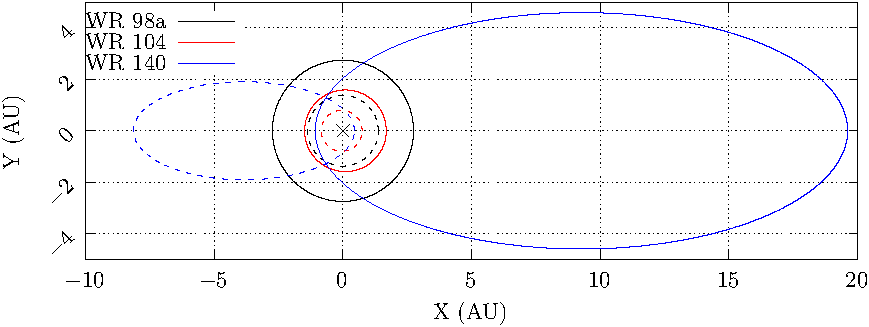
\includegraphics[width=\linewidth]{assets/orbits-crop.pdf}
  \caption[System orbital paths]{Comparative orbital paths of each system about a common barycenter at (0,0), solid lines represent the WR star in the binary system, whilst dashed lines represent the OB star. WR 140 is notable for having a highly eccentric orbit, and thus a significantly longer orbital period.}
  \label{fig:orbits-diag}
\end{figure}

% Discussion of WR 98a
WR 98a is a typical dusty CWB system that was primarily chosen for simulation as it is one of the only CWB systems whose dust dynamics have been simulated in an academic paper \parencite{hendrix_pinwheels_2016}. The model utilised in Hendrix et al. was a dual-fluid model with an Epstein drag function in order to detail how dust flows through the system itself. As such, this model does not simulate dust accretion or cooling, and only deposits dust grains with a single set grain radius and a fixed dust production rate of $\phi = 0.0763$. However, this still provides a useful point of comparison to evaluate this papers dust model against an established model with concrete data. Furthermore, a simplified version of WR 98a was used to test the dust model and was used as a basis to explore the parameter space of dusty CWB systems by varying wind parameters and orbital separation. The parameters detailed in table \ref{tab:systems-wind-properties} are adopted from Hendrix et al., similarly to this paper a perfectly circular orbit is assumed.

% Discussion of WR 104

WR 104 is an archetypical dust forming binary system that is extensively observed, with multiple papers on the dynamics and formation of dust in the system. %//TODO cite this

WR 104 represents the high end of dust formation in CWB systems, with a high dust formation rate in the order of \num{3e-7} \si{\solarmass\per\year}, the close separation of the binary system combined with the high mass loss rate results in a much lower value of $\chi$ for the WR wind, suggesting very strong cooling in the post-shock wind collision region. As such this system is more difficult to simulate, as a higher resolution and lower Courant number are required in order to reliably simulate the post-shock cooling effect.
%//TODO CITE
The orbital and wind parameters of this system were derived from \cite{soulain_sphere_2018} and \cite{harries_three-dimensional_2004}. 

% Talking points on similarities and differences between WR 104 and WR 140


% Discussion of WR140

WR 140 was simulated for this experiment as it represents an archetypical episodic CWB system, whose infrared dust emission peaks around periastron passage. WR 140 deviates from WR 98a and WR 104 by being extremely eccentric, which significantly effects the cooling parameter as the orbit progresses (figure \ref{fig:chiphase}). Additionally, the minimum value for $\chi$ is significantly larger than the other systems, and hence cooling would be less dominant on the dynamics of the WCR, even at periapsis. Though these simulations do not calculate wind acceleration due to radiative line driving, both stellar winds are expected to be accelerated close to their terminal wind velocities \parencite{lamersIntroductionStellarWinds1999}. However, this discrepancy should be noted when considering the results of this paper. %//TODO touch up 
The orbital and wind parameters of this system were derived from work by \cite{monnier_first_2011}, \cite{usov_stellar_1991}, as well as \cite{thomasOrbitStellarMasses2021}.

\begin{figure}[h]
  \centering
  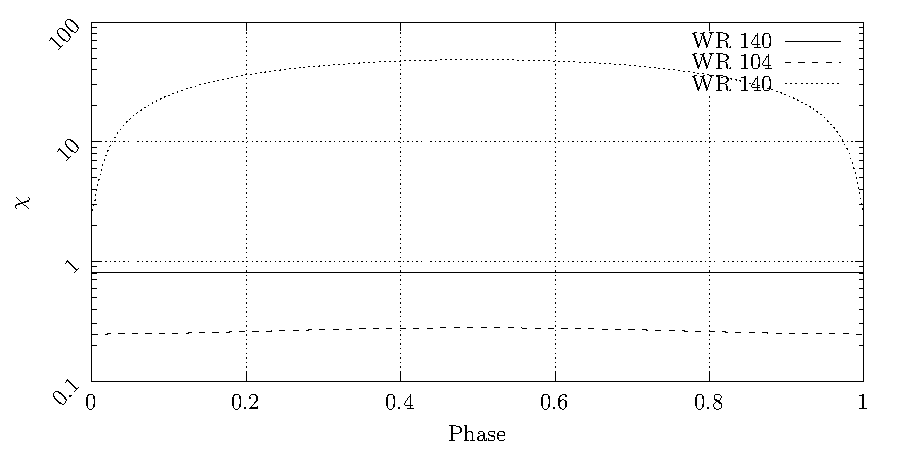
\includegraphics[width=\linewidth]{assets/chi-vs-phase.pdf}
  \caption[$\chi_{WR}$ change over system orbit]{Change in WR cooling parameter $\chi_{WR}$ as system orbits, the dynamics of the WCR for WR 98a and WR 104 is dominated by cooling throughout their entire orbits, while WR 140 is adiabatic for most of its orbit.}
  \label{fig:chiphase}
\end{figure}


% Challenges involved in simulating WR140
%//TODO Check if this is right

Significant challenges are involved in simulating the WR 140 system compared to the other systems in this paper. The highly eccentric orbit of this system means that in order to simulate a full orbit of this system, a large section of the simulation would need to be rendered at full resolution, resulting much shorter timesteps and a significantly larger processor and memory requirement. This is impractical considering the time constraints of this project. In order to alleviate this issue the system was simulated with Adaptive Mesh Refinement (AMR) conditions instead of SMR. The region surrounding the stars orbit was refined and de-refined in order to ensure that there were at least 128 cells of finest size separating the stars. Additional refinement rules were established to progressively lower the grid resolution further out from the stars, as well as to ensure that the collision region was properly resolved.

%//TODO Is it still 128? Check logic for other conditions

%//TODO Am I still even using AMR? WRitten when not established, but this was the intent

%//TODO Check to see if uncertainty in any of the systems

%//TODO discuss refinement conditions, maybe even a pseudocode section?

\subsection{Radiative transfer modelling}
